\documentclass[aps,pra,12pt,notitlepage,tightenlines]{revtex4-1}
%\usepackage[margin=2.5cm]{geometry}
\usepackage{amsmath,amssymb,textcomp,graphicx,url,bm,lipsum,hyperref,color,subcaption,afterpage,gensymb}

\newcommand\matr[1]{\bm{#1}}
\newcommand\barparen[1]{\overset{\textbf{\fontsize{5pt}{5pt}\selectfont(---)}}{#1}}

\graphicspath{{Images/}}

\begin{document}

\title{Upgrading T2K and an Overview of Electron Neutrino Detection in ND280\vspace{0mm}}
\author{Wilf Shorrock\vspace{1mm}}
\affiliation{Imperial College London\vspace{-0.5mm}}
\date{\today}
\begin{abstract}
\linespread{0.97}
\vspace{1mm}The T2K experiment is set to enter a new phase of data-taking in 2020, with increased statistics. To make full use of the higher statistics and reduce systematic errors, upgrades to the near detector, ND280, have been proposed. In this report, after introducing the T2K experiment and describing the sub-detectors comprising ND280, the updates to ND280's hardware and software will be outlined. The beam tests performed at CERN for the prototypes of the upgraded detectors will also be described, with particular focus on the Super-FGD prototype. A description of the detection of electron neutrinos at ND280 will also be included, as an introduction to the future work I will be carrying out for my PhD.
\end{abstract}

\maketitle

\newpage
\tableofcontents
\newpage

\vspace{-8mm}

\section{Introduction}
In their 1956 paper announcing the discovery of the neutrino, Reines and Cowan stated:
\begin{quotation}
 ``Each new discovery of natural science broadens our knowledge and deepens our understanding of the    physical universe; but at times these advances raise new and even more fundamental questions than those     which they answer~\cite{1956Natur.178..446R}.''
\end{quotation}
At the time, they were referring to the observation of beta decay and how it led to the proposal of the neutrino, but it is rather fitting that we can also apply this statement to the neutrino itself. Since the observation of atmospheric neutrino oscillations at Super-Kamiokande (SK) in the 1990s, a whole new area of research has opened up, and results from further experiments observing reactor neutrinos~\cite{PhysRevLett.108.171803, PhysRevLett.108.191802, PhysRevLett.108.131801} have shown that neutrinos oscillate between three flavour states via three mass eigenstates. 

Neutrino oscillation has become one of the more promising avenues towards Beyond Standard Model physics. It has also been used to explain the lack of electron neutrinos originating from the Sun, a problem that had been present since the 1960's~\cite{PhysRevLett.89.011301}. Present-day experiments are still trying to make more precise measurements of the oscillation parameters, and are also trying to ascertain whether Charge Parity (CP) is conserved or not in these oscillations.

Tokai to Kamioka (T2K) is a long-baseline experiment that studies accelerator neutrinos, which are produced as the tertiary products of high energy protons striking a graphite target. T2K began operation in 2010 with the goal of making precision measurements of the oscillation parameters $\Delta m^2_{23}$ and $\sin^22\theta_{23}$ and a first measurement of the mixing angle $\theta_{13}$ (these parameters are explained in Sec.\ \ref{sec:osc})~\cite{PhysRevD.88.032002}. It has been successful in these goals, with its most recent results published in 2017~\cite{Abe:2017bay}. Over the next few years, the experiment will attempt to observe CP violation (CPV) in neutrino oscillations with at least a 3$\sigma$ significance (if the CPV is maximal) and ascertain whether the mixing angle $\theta_{23}$ is maximal, as current measurements suggest. This new phase of the experiment will be called T2K-II and will require several upgrades to the experiment's detectors.

This paper will provide an overview of the proposed upgrade to the T2K experiment's off-axis near detector, ND280. The process of analysing the near detector's data to ascertain the electron neutrino contamination of the neutrino beam will also be presented, with the goal of introducing the future work of the author. Firstly, though, the theory behind neutrino oscillation will be given, leading on to a description of the T2K experiment and details on the current structure of ND280 and it's software.

\section{Neutrino Oscillation Model}
\label{sec:osc}
Disregarding sterile neutrinos, neutrino oscillations are well described by the Pontecorvo-Maki-Nakagawa-Sakata (PMNS) matrix. This PMNS matrix relates the three neutrino flavour eigenstates, $(\nu_e, \nu_\mu, \nu_\tau)$, to three mass eigenstates, $(\nu_1, \nu_2, \nu_3)$, through the equation

\begin{gather}
\label{eq:pmns}
 \begin{pmatrix}
 \nu_e \\
 \nu_\mu \\
 \nu_\tau 
 \end{pmatrix}
 =
 \begin{bmatrix}
 U_{e1} & U_{e2} & U_{e3} \\
 U_{\mu1} & U_{\mu2} & U_{\mu3} \\
 U_{\tau1} & U_{\tau2} & U_{\tau3}
 \end{bmatrix}
 \begin{pmatrix}
  \nu_1 \\
 \nu_2 \\
 \nu_3 
 \end{pmatrix}
 ,
\end{gather}
where the matrix enclosed by square brackets is the PMNS matrix, $\matr{M}_\mathrm{PMNS}$. The matrix elements $U_{\alpha i}$ represent the mixing amplitudes of mass state $i$ contained within flavour state $\nu_\alpha$.

Eq.\ \eqref{eq:pmns} shows that the flavour eigenstates are coherent superpositions of the mass eigenstates. This means that, following the weak decay $W \rightarrow l_\alpha\nu_\alpha$, where $\nu_\alpha$ is a neutrino flavour eigenstate and $l_\alpha$ is the corresponding charged lepton state with flavour $\alpha$, the neutrino will propagate as a mixture of the mass eigenstates, which interfere quantum mechanically in interactions. This allows the neutrino to interact later in time as if it had a different flavour, where the probability of this flavour is dependent on the distance the neutrino travelled~\cite{Kayser:2005cd}. 

Because the matrix is a unitary $3\times3$ matrix, $\matr{M}_\mathrm{PMNS}$ can be parametrised using three real angles, $(\theta_{12}, \theta_{13}, \theta_{23})$, and a real phase, $\delta_\mathrm{CP}$, to give
\begin{gather}
 \matr{M}_\mathrm{PMNS} = 
 \begin{bmatrix}
 1 & 0 & 0 \\
 0 & C_{23} & S_{23} \\
 0 & -S_{23} & C_{23}
 \end{bmatrix}
 \begin{bmatrix}
 C_{13} & 0 & S_{13}e^{-i\delta_\mathrm{CP}} \\
 0 & 1 & 0 \\
 -S_{13}e^{i\delta_\mathrm{CP}} & 0 & C_{13}
 \end{bmatrix}
 \begin{bmatrix}
 C_{12} & S_{12} & 0 \\
 -S_{12} & C_{12} & 0 \\
 0 & 0 & 1
 \end{bmatrix}
 ,
\end{gather}
where $C_{ij} = \cos\theta_{ij}$ and $S_{ij} = \sin\theta_{ij}$. These parameters are useful in defining the probabilities of neutrino oscillations; hence it is these parameters that oscillation experiments aim to measure. A non-zero value of the $\delta_{CP}$ phase (given that $S_{13}\neq 0)$ would mean that neutrino oscillations are CP-violating. There may be two extra phase parameters required if neutrinos are Majorana particles---i.e.\ if the neutrino is its own antiparticle---but these have no effect on oscillation measurements~\cite{Kayser:2005cd}.

We will not go into the details of the derivation of neutrino oscillation probabilities here, but we will quote the notation from Kayser~\cite{Kayser:2011jn}, where he gives the probability of a (anti-)neutrino with initial flavour $\alpha$ and energy $E_\nu$ propagating a distance $L$ and being detected with flavour $\beta$ as:
\begin{align}
\label{eq:p}
P\Big(\barparen{\nu_\alpha}\rightarrow\barparen{\nu_\beta}\Big) = \delta_{\alpha\beta}&-4\sum^3_{i<j}\Re[U_{\alpha i}U_{\beta i}^*U_{\alpha j}^*U_{\beta j}]\sin^2\bigg(\Delta m^2_{ij}\frac{L}{4E_\nu}\bigg) \notag \\
& \mp 2\sum^3_{i<j}\Im[U_{\alpha i}U_{\beta i}^*U_{\alpha j}^*U_{\beta j}]\sin\bigg(\Delta m^2_{ij}\frac{L}{2E_\nu}\bigg),
\end{align}
where $\Delta m^2_{ij} = m^2_i - m^2_j$ is the difference between the squared masses of mass eigenstates $i$ and $j$. 

Eq.~\ref{eq:p} can only be applied to neutrinos travelling through a vacuum. For neutrino propagation through matter, see the report by Kayser~\cite{Kayser:2005cd}.

\section{T2K}
T2K uses a neutrino beam that is generated at the Japan Proton Accelerator Research Complex (J-PARC) in Tokai. The beam crosses the breadth of the main Japanese island, Honshu, from Tokai on the east coast to Kamioka on the west coast, travelling in a straight line through the Earth's crust. In Tokai, the beam passes through two near detectors---INGRID and ND280---that are 280~m from the beam's origin. At Kamioka, the beam reaches the far detector, SK, 295~km from the origin. An illustration of the experiment is shown in Fig.\ \ref{fig:t2k}.
\begin{figure}
 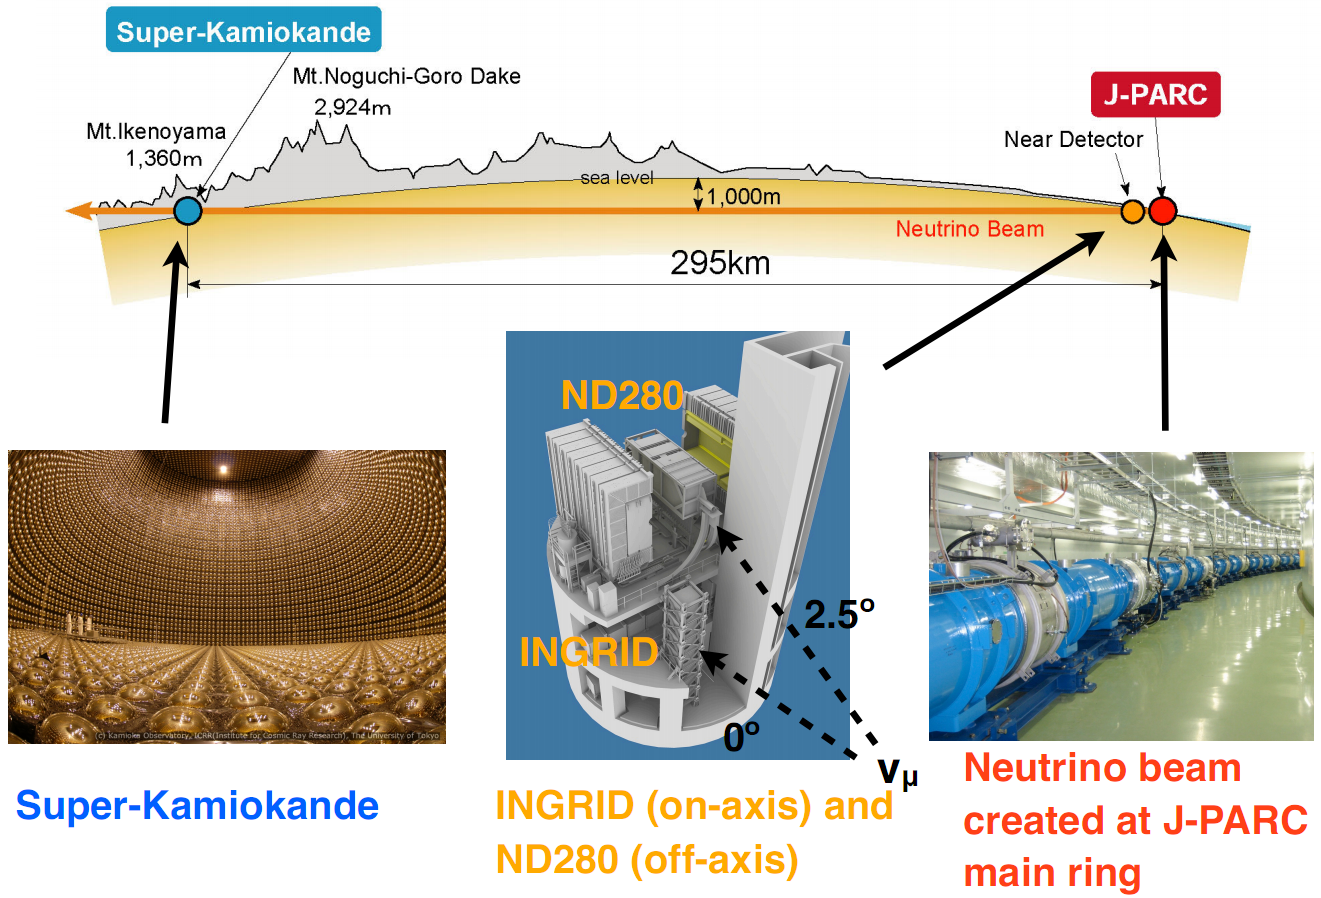
\includegraphics[scale=0.33]{T2K_detail}
 \caption{A diagram showing the journey of the neutrino beam produced in the T2K experiment, along with illustrative photos of each major stage of the beam. The beam originates at J-PARC, then passes through the two near detectors, INGRID and ND280, which are on- and off-axis respectively. After travelling 295~km the beam then passes through the Super-Kamiokande water cherenkov detector, which is also off-axis~\cite{Jamieson:2015rza}.}
 \label{fig:t2k}
\end{figure}

The INGRID detector lies on the axis of the neutrino beam, but ND280 and SK are 2.5\degree\ off-axis, which sets the peak of the neutrino flux at 600~MeV, the energy at which muon neutrino disappearance is most likely. Fig.\ \ref{fig:axis} 
\begin{figure}
 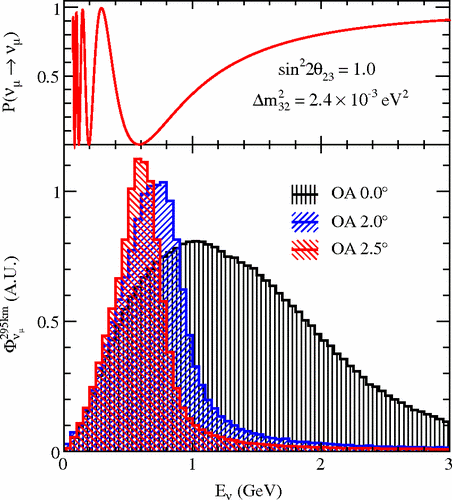
\includegraphics[scale=0.5]{axis.png}
 \caption{A probability plot (top) of the probability of muon neutrino survival as a function of energy, and a plot of the neutrino beam energy flux (bottom) for several off-axis angles.}
 \label{fig:axis}
\end{figure}
shows the flux of the neutrino beam as a function of neutrino energy, at several different off-axis angles. Also shown is the probability of a muon neutrino not oscillating as a function of neutrino energy. It is clear that the peak flux for a 2.5\degree\ off-axis angle occurs at the same energy as one of the minimum points in the probability plot.

In this report, we will only give details on the ND280 detector and its proposed upgrades. Information on the other detectors and the beamline is given elsewhere~\cite{ABE2011106}.

\section{ND280: Current State}
ND280, so called because it is a Near Detector 280~m away from the neutrino beam's origin, measures the flux, the energy spectrum, and the flavour content of the neutrino beam. This allows comparison with measurements at the far detector, leading to calculations of neutrino oscillation parameters by observing how the flavour content of the beam has changed as a function of energy. 

As well as monitoring the beam characteristics, ND280 also takes data for neutrino cross-section measurements, which helps provide a more accurate oscillation analysis. 

The detector itself can be broken down into three main systems: a $\pi^0$ detector (P\O D), a tracker consisting of several fine grain detectors (FGDs) and time-projection chambers (TPCs), and an electromagnetic calorimeter (ECal). The whole detector is subject to a 0.2 T magnetic field for particle identification and momentum determination (see Fig.\ \ref{fig:ND} for visualisation).
\begin{figure}
 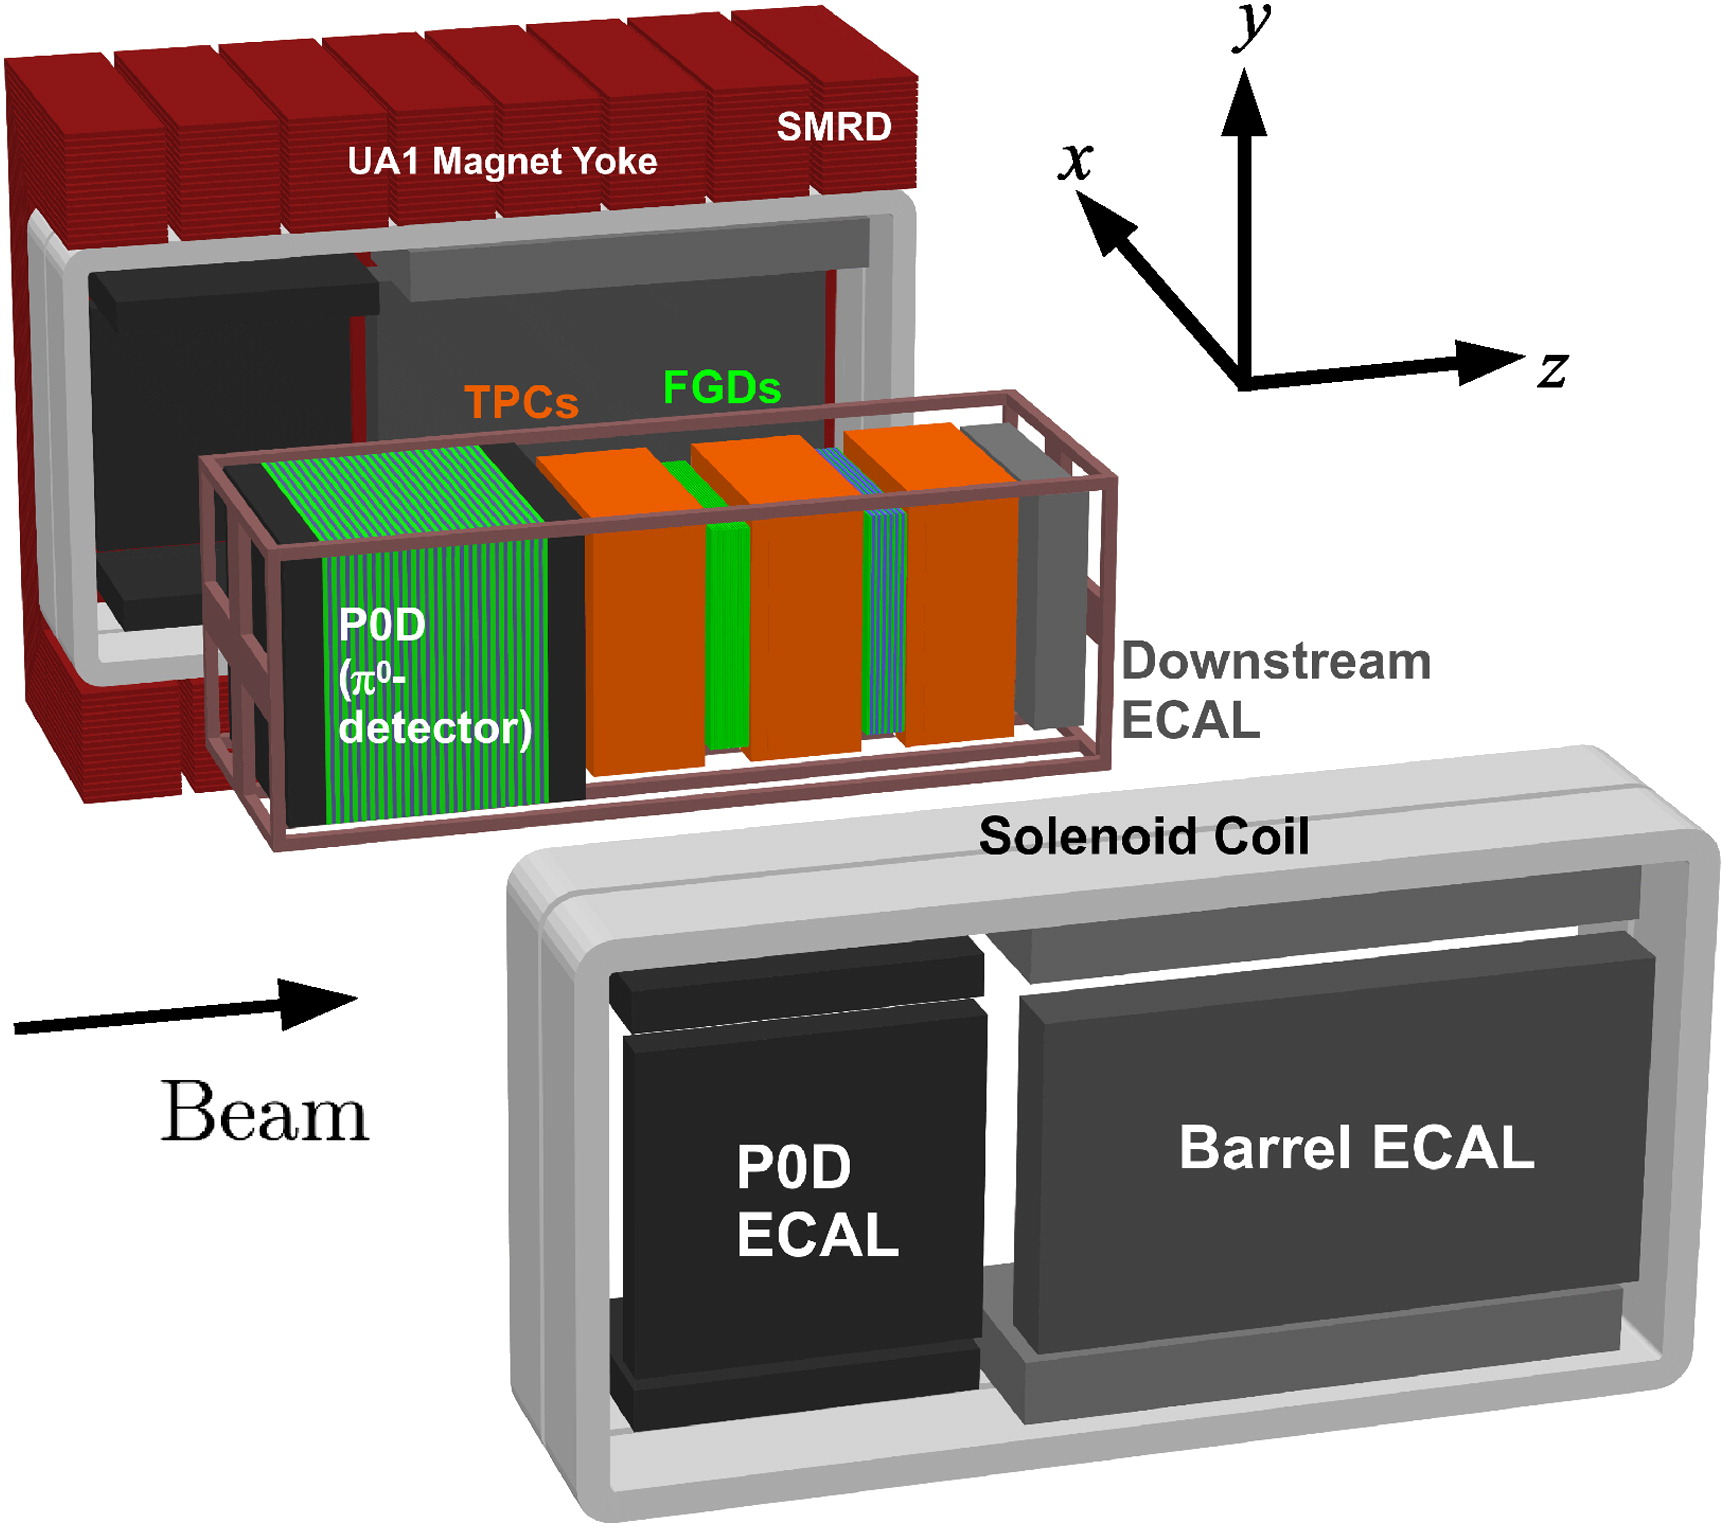
\includegraphics[scale=1]{ND280.png}
 \caption{Expanded view of the ND280 detector, showing the positions of each of the three main sub-systems. The entire detector is encased in the UA1 magnet with a 0.2~T magnetic field~\cite{ABE2011106}.}
 \label{fig:ND}
\end{figure} 

\subsection{$\pi^0$ Detector (P\O D)}
Neutral pions are a major source of uncertainty at T2K, as they can be misidentified as electrons in SK. To reduce the uncertainty caused by these misidentifications, the P\O D is used to measure the cross-sections of neutrino interactions, specifically with water, where a $\pi^0$ appears in the final state. Using this cross-section data, the number of $\pi^0$s produced in SK can then be calculated and taken into account.

The detector has a central water target, which constitutes alternating layers of brass, scintillator, and fillable water target bags. This central target is preceded and followed by electromagnetic calorimeters, comprised of alternating sheets of lead and scintillator. The ECals are used for rejecting particles entering the P\O D that originated from outside the detector, and also to contain and measure electromagnetic showers. Cross-section values can be deduced by taking measurements when the target bags in the central water target are filled with water and comparing them to when they are empty~\cite{ABE2011106, Assylbekov:2011sh}.

\subsection{Fine Grain Detectors (FGDs)}
The FGDs provide mass with which incoming neutrinos can interact. They also provide precision tracking to map out the interaction vertices. They consist of bars of scintillator, oriented perpendicular to the neutrino beam, stacked to form layers. Two layers are attached together to form a module, with the bars of one layer being arranged vertically, and the other layer horizontally. This allows precise determination of particle position in two dimensions.

There are two FGDs in ND280. The downstream FGD also contains layers of water in between the scintillator layers. Comparing interaction rates between the two FGDs allows calculation of the cross-sections of neutrino interactions with carbon and water~\cite{ABE2011106, Amaudruz:2012agx}.

\subsection{Time Projection Chambers (TPCs)}
There are three TPCs in ND280, sandwiching the two FGDs. The bulk of each TPC consists of an argon-based gas. When charged particles pass through this gas, they ionise the gas molecules. The ionisation electrons drift away from a cathode and towards a readout plane. The location and arrival time of the electrons on this plane can be used to construct a 3D image of the particle's trajectory.

TPCs are ideal for identifying the number and trajectory of charged particles in the detector. This allows selection of low-contamination interaction samples, as well as momentum measurements from curved tracks caused by the magnetic field present in the detector. Combining the particle momenta along with the ionisation of the particle tracks, one can identify the type of charged particle that made each track. Hence, when combined with the FGD data, the TPCs can be used to help estimate the neutrino flux as a function of energy, and to determine the contamination in the neutrino beam by electron neutrinos~\cite{ABE2011106, Abgrall:2010hi}.

\subsection{Electronic Calorimeter (ECal)}
As well as the ECals either end of the P\O D, there are also ECals surrounding the entire detector. A barrel ECal surrounds the tracker, another ECal is situated downstream of the tracker, and a third encircles the P\O D. %These ECals are arranged to try and minimise the number of particles that leave the detector without passing through an ECal. 

The main uses of the ECals are to complement the inner detectors by measuring the energies of photons missed by the inner detectors, reject particles from interactions outside the detector, and help with particle identification.

Alternating layers of scintillator and lead absorber make up each ECal. The scintillator layers consist of several bars of plastic scintillator. These bars are oriented perpendicular to the scintillator bars of the adjacent layers for $x$--$y$ tracking~\cite{ABE2011106, Allan:2013ofa}.

\subsection{ND280 Software}
The ND280 software is used for offline analysis of data collected by ND280, as well as Monte Carlo (MC) data generation and analysis. The basic framework of the code was built in 2004, with the underlying structure and data storage relying on ROOT~\cite{Brun1997}, simulation libraries from Geant4~\cite{Agostinelli2003}, a package management system provided by CMT (Configuration Management Tool) \cite{Arnault:2000vu} and the version control system used to store each version of the code is CVS (Concurrent Version Systems) \cite{Berliner2001}.

A decision was made early-on in the software's lifetime to split the structure of the software into different packages, resulting in about 60 software packages in total~\cite{ABE2011106}. This offers easy access to specific areas of code and makes editing the software simpler for developers. 

The flow-path of the different data types through the package structure is shown in Fig.\ \ref{fig:struct} (only the most relevant packages are shown). 
\begin{figure}
 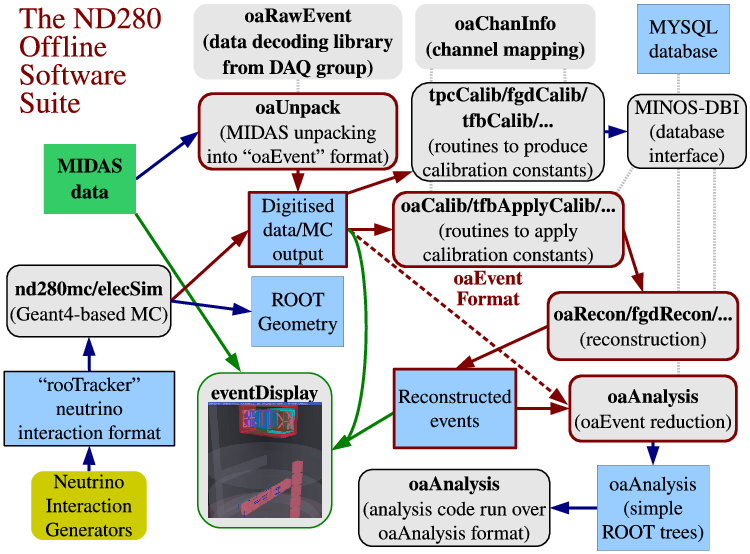
\includegraphics[scale=0.5]{struct.png}
 \caption{The flow of data through the package structure of the ND280 software. The flow is simplified and only shows the most relevant packages. Boxes with red coloured borders represent packages that process oaEvent data.~\cite{ABE2011106}}
 \label{fig:struct}
\end{figure}
The package oaEvent is important as it defines the format of the data passed through the software between the steps where raw MIDAS data (MIDAS is the format of data from the ND280 detector \cite{Ritt2001}) is passed to the software and the final step where oaAnalysis reduces the data to a user-friendly format. The oaUnpack and oaRawEvent packages handle the conversion of MIDAS data to oaEvent data. oaCalib then applies calibration constants to the data, whilst oaCalib's sub-packages use the data to produce calibration constants to store in MYSQL to be used by oaCalib. The data is then passed on to oaRecon, which uses the data to reconstruct the particle events that occurred in the detector, the results of which are analysed by oaAnalysis.

The exact same processes are applied to MC data, except that the data does not start in MIDAS format. The MC data is produced by passing information from the neutrino flux packages to the neutrino interaction generators NEUT~\cite{Hayato:2009zz} and GENIE~\cite{Andreopoulos2010}. These generators produce realistic distributions of child particles from neutrino interactions. The simulation is then taken over by nd280mc, which uses Geant4 to propagate the child particles and simulate the energy deposits left in the detector. elecSim then converts these energy deposits to simulated electrical readouts, as would be seen in the real detector and recorded in MIDAS format, except here it is written as oaEvent data.
 
\section{Hardware Upgrades}
Resulting from T2K's success in measuring oscillation parameters with improved precision, the experiment is set for a series of upgrades to further increase the measurement precision. In tandem with these improvements, ND280 must also be revamped to reduce statistical and systematic uncertainties in the neutrino appearance predictions. Here, we will go through the proposed upgrades, which are planned for construction over 2019--2020 to be installed in Japan in 2020~\cite{Blondel:2299599}.

The proposed upgraded ND280 is shown in Fig.\ \ref{fig:up}.
\begin{figure}
 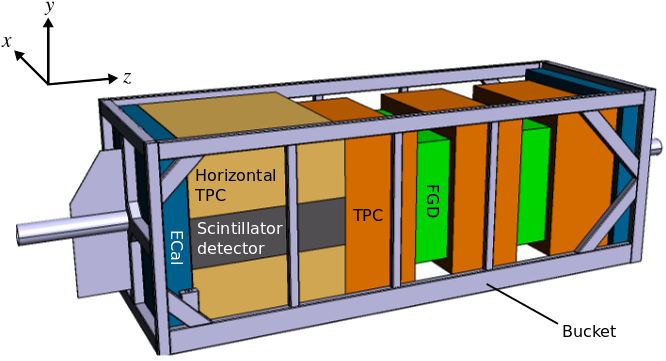
\includegraphics[scale=0.5]{upgrade2.png}
 \caption{The proposed upgrade of ND280. The new additions are the horizontal TPCs (light brown) and the scintillator detector (grey), which replace the P\O D. The ``bucket'' is a framework that supports the detectors. Not shown are the barrel ECals that will surround the detectors, similar to the original design. The neutrino beam propagates in the $z$ direction~\cite{Blondel:2299599}.}
 \label{fig:up}
\end{figure}
The downstream end of the detector will remain unchanged, with three TPCs separated by two FGDs. At the upstream end, however, the central P\O D module (not the ECal endcaps) will be replaced by a scintillator detector sandwiched between two horizontal TPCs. The scintillator detector will act as a target material, with the TPCs distributed around it giving nearly 4$\pi$ solid angle coverage. This  will address an issue with the old ND280 design: the tracking efficiency is biased towards low scattering angles. This is because, after a neutrino has interacted in an FGD, the resulting lepton is only seen in the downstream TPC if the scattering angle is less than $\sim$40\degree\ with respect to the beam direction. The TPC gives important information on the interaction, so most interaction samples exclude leptons with high scattering angles. This creates problems when comparing data with SK, which has a flat efficiency with respect to scattering angle.

The new scintillator detector will have a first-of-its-kind ``Super-FGD'' design that incorporates scintillator cubes rather than bars, which can be read out from three orthogonal directions by wavelength shifting (WLS) fibres. The cubes' side length will be between 1--2~cm, with the larger lengths sacrificing granularity for a smaller number of cubes and readouts. The size of the cubes is comparable to the height and width of the scintillator bars used in the current design, but the bars only give readouts in two directions. The extra information provided by the cubes helps to reconstruct the paths of multiple particles. Fig.~\ref{fig:sfgd}
 \begin{figure}
  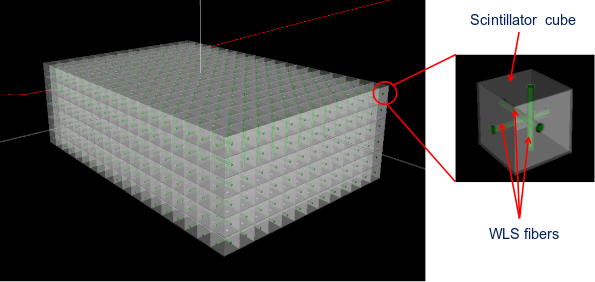
\includegraphics[scale=0.75]{SFGD.png}
  \caption{A rendering of the Super-FGD to be used in the upgraded ND280. The detector comprises many small plastic scintillator cubes that are read off in three orthogonal directions by wavelength shifting fibres. There are fewer cubes depicted here than there will be in the actual detector, to make the diagram clearer~\cite{Blondel:2299599}.}
  \label{fig:sfgd}
 \end{figure}
shows an illustration of the Super-FGD design.

Not shown in the diagram of the ND280 upgrade (Fig.\ \ref{fig:up}) are the new Time-Of-Flight (TOF) detectors that are to be installed. These will be placed around the volume containing the scintillator detector and the horizontal TPCs. The TOF detectors will help identify whether a particle originated from inside or outside the detector, and will also aid with particle identification. The design of the TOF detectors is as yet undecided. There are two possible candidates, one based on wavelength shifting fibres and the other based on plastic scintillator bars. A prototype of the latter design is being constructed in 2018 and will be used in conjunction with the test-beam that will be run at the end of 2018. Prototypes of the horizontal TPC and the Super-FGD will also be used in the test-beam, the latter of which will be explained in more detail in the next section.

\section{Super-FGD Beam Test}
The beam test for the Super-FGD prototype is scheduled for June 27th -- July 11th 2018, taking place at CERN. At the time of submission for this report the beam test will be partially completed, making it difficult to report results. I will be at CERN for the beam test and the weeks preceding it, so I will report on the set-up of the beam test, the prototype's design and the initial results, as well as describing my specific roles in the preparation and testing.

\subsection{The Super-FGD Prototype}
The prototype scintillator detector measures $24\times48\times8$ cm$^3$ and comprises 9216 extruded polystyrene mixed with p-terphenyl plastic scintillator cubes, each 1~cm long. There are a total of 1728 WLS fibres threaded through the cubes. On one end of each fibre is a connector, which attaches to another connector in which is housed a Multiple Photon Pixel Counter (MPPC) that sends a signal down a length of cable to a circuit board where the signal is processed //MORE DETAIL. Two photographs of the prototype are shown in Fig.\ \ref{fig:proto},
 \begin{figure}
  \centering
  \begin{subfigure}{.5\textwidth}
   \centering
   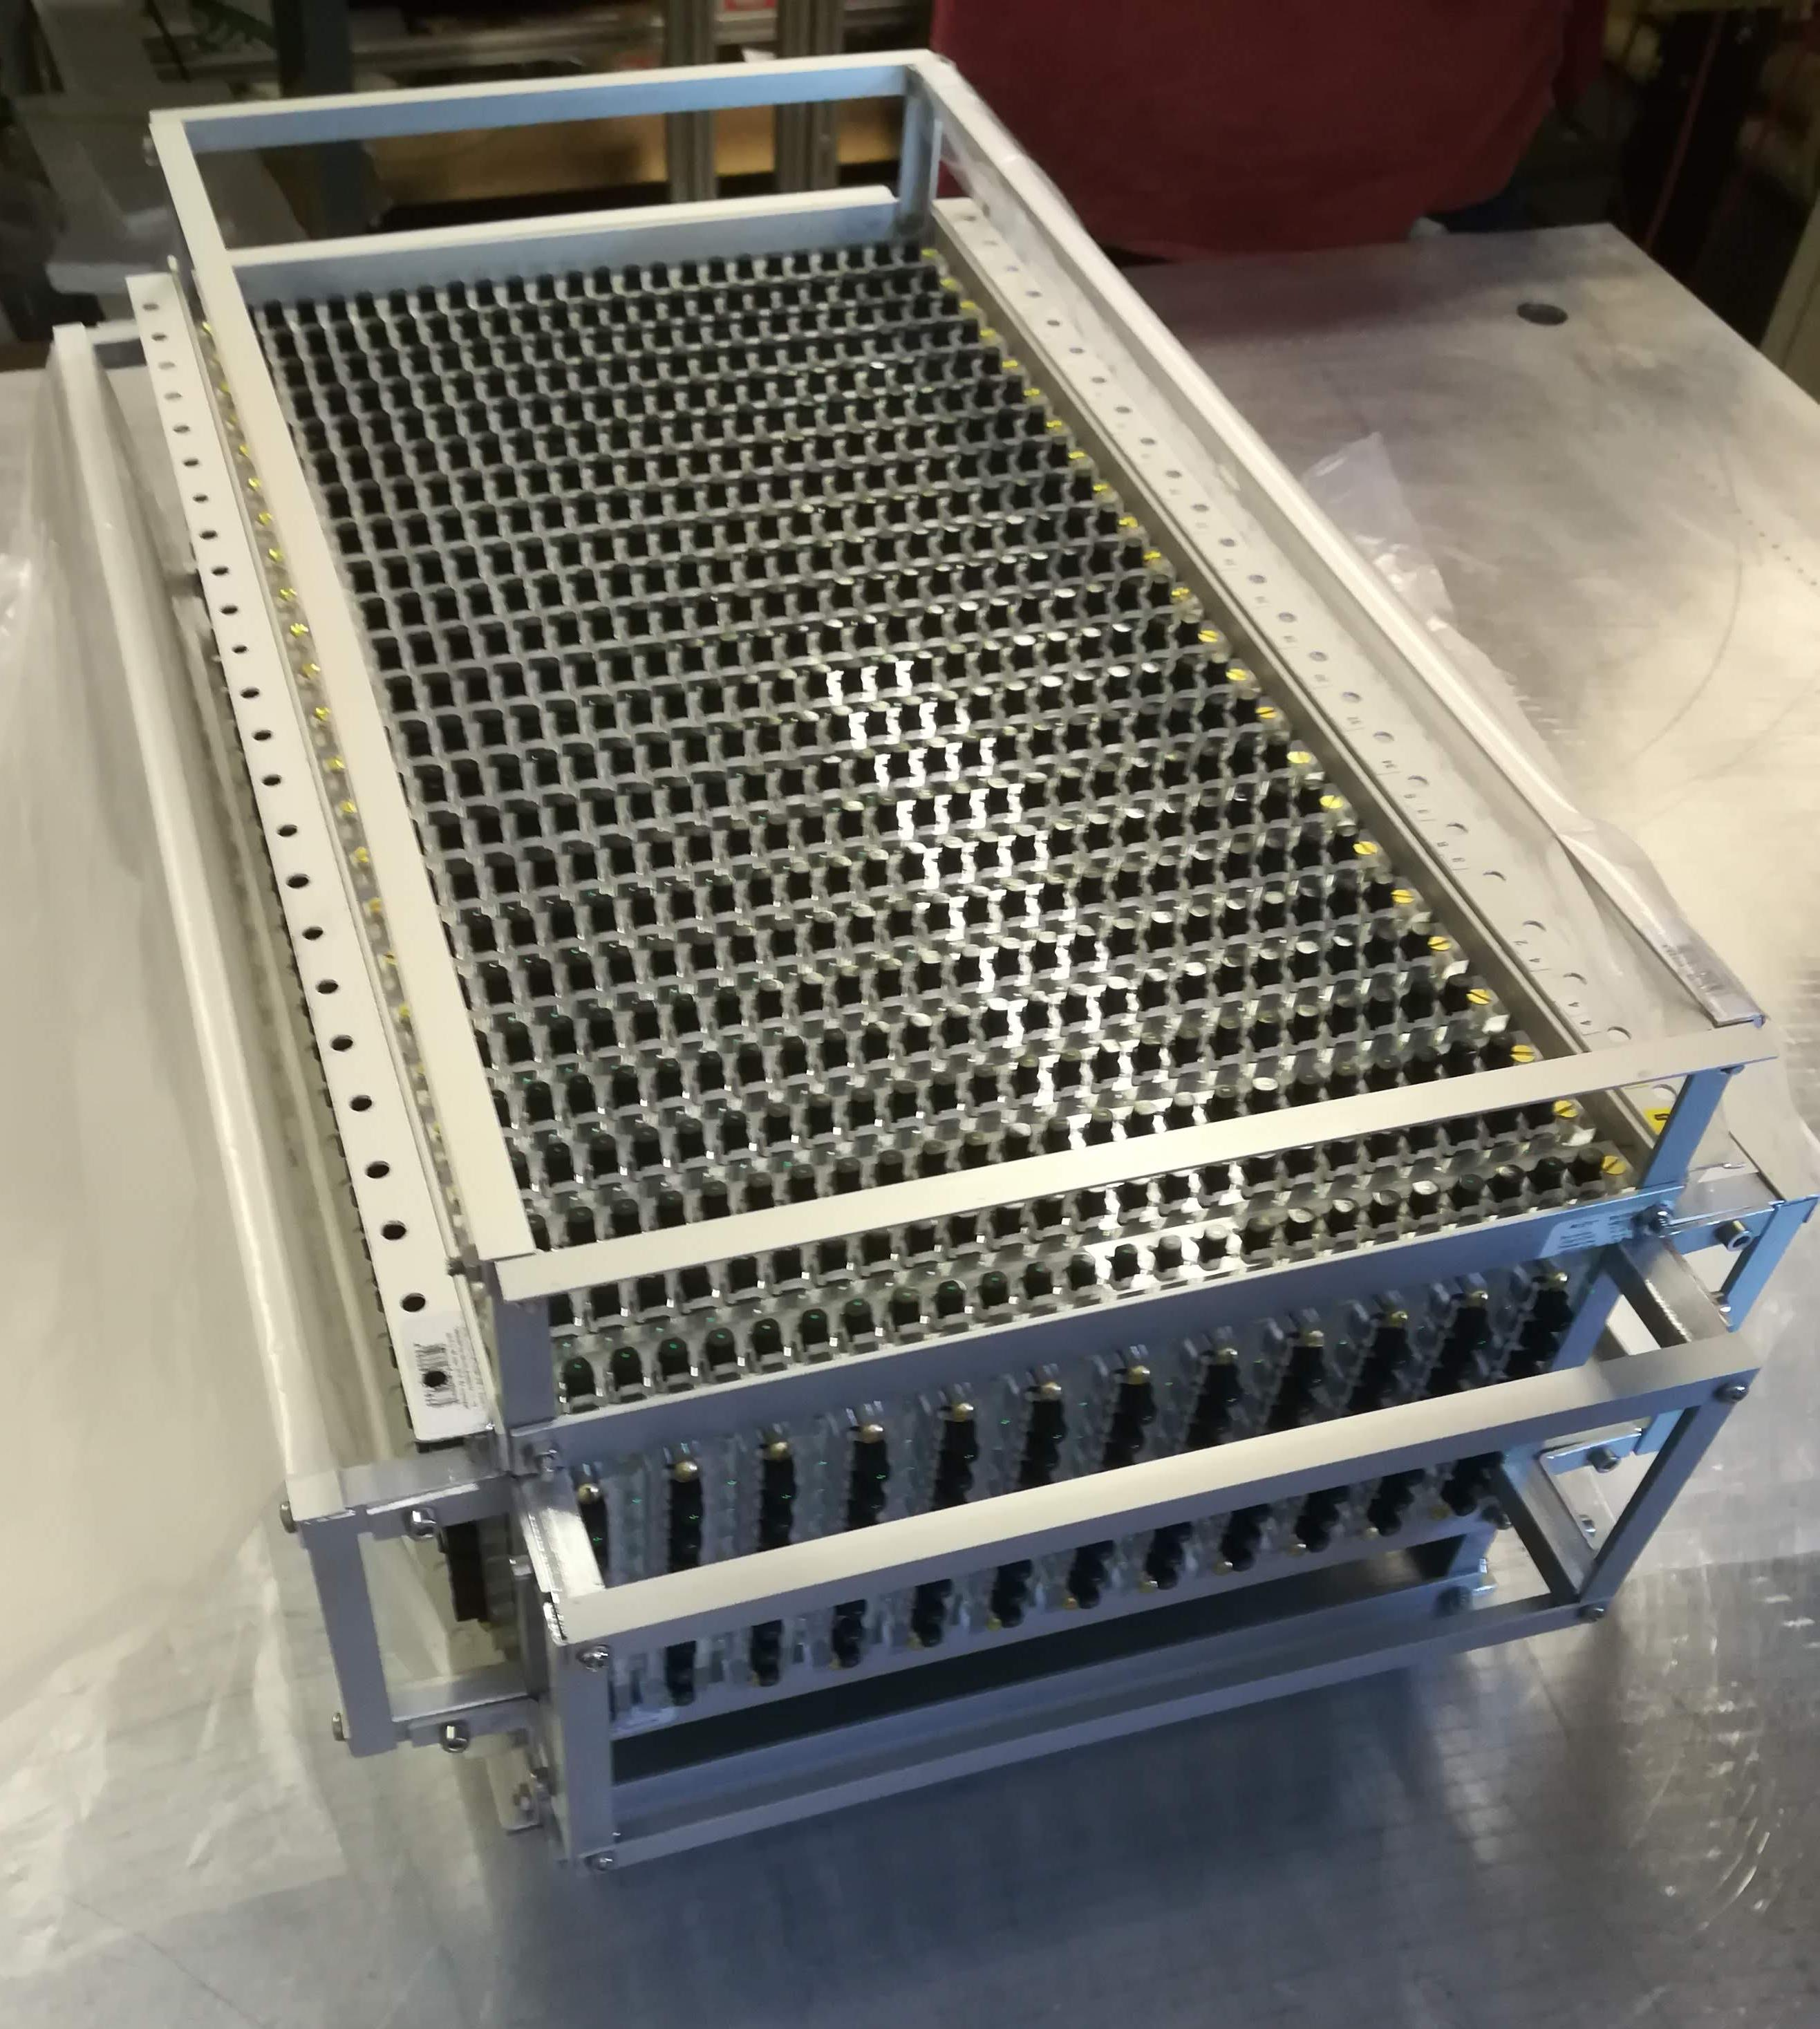
\includegraphics[width=.7\linewidth]{proto}
   \caption{•}
   \label{protoa}
  \end{subfigure}%
  \begin{subfigure}{.5\textwidth}
   \centering
   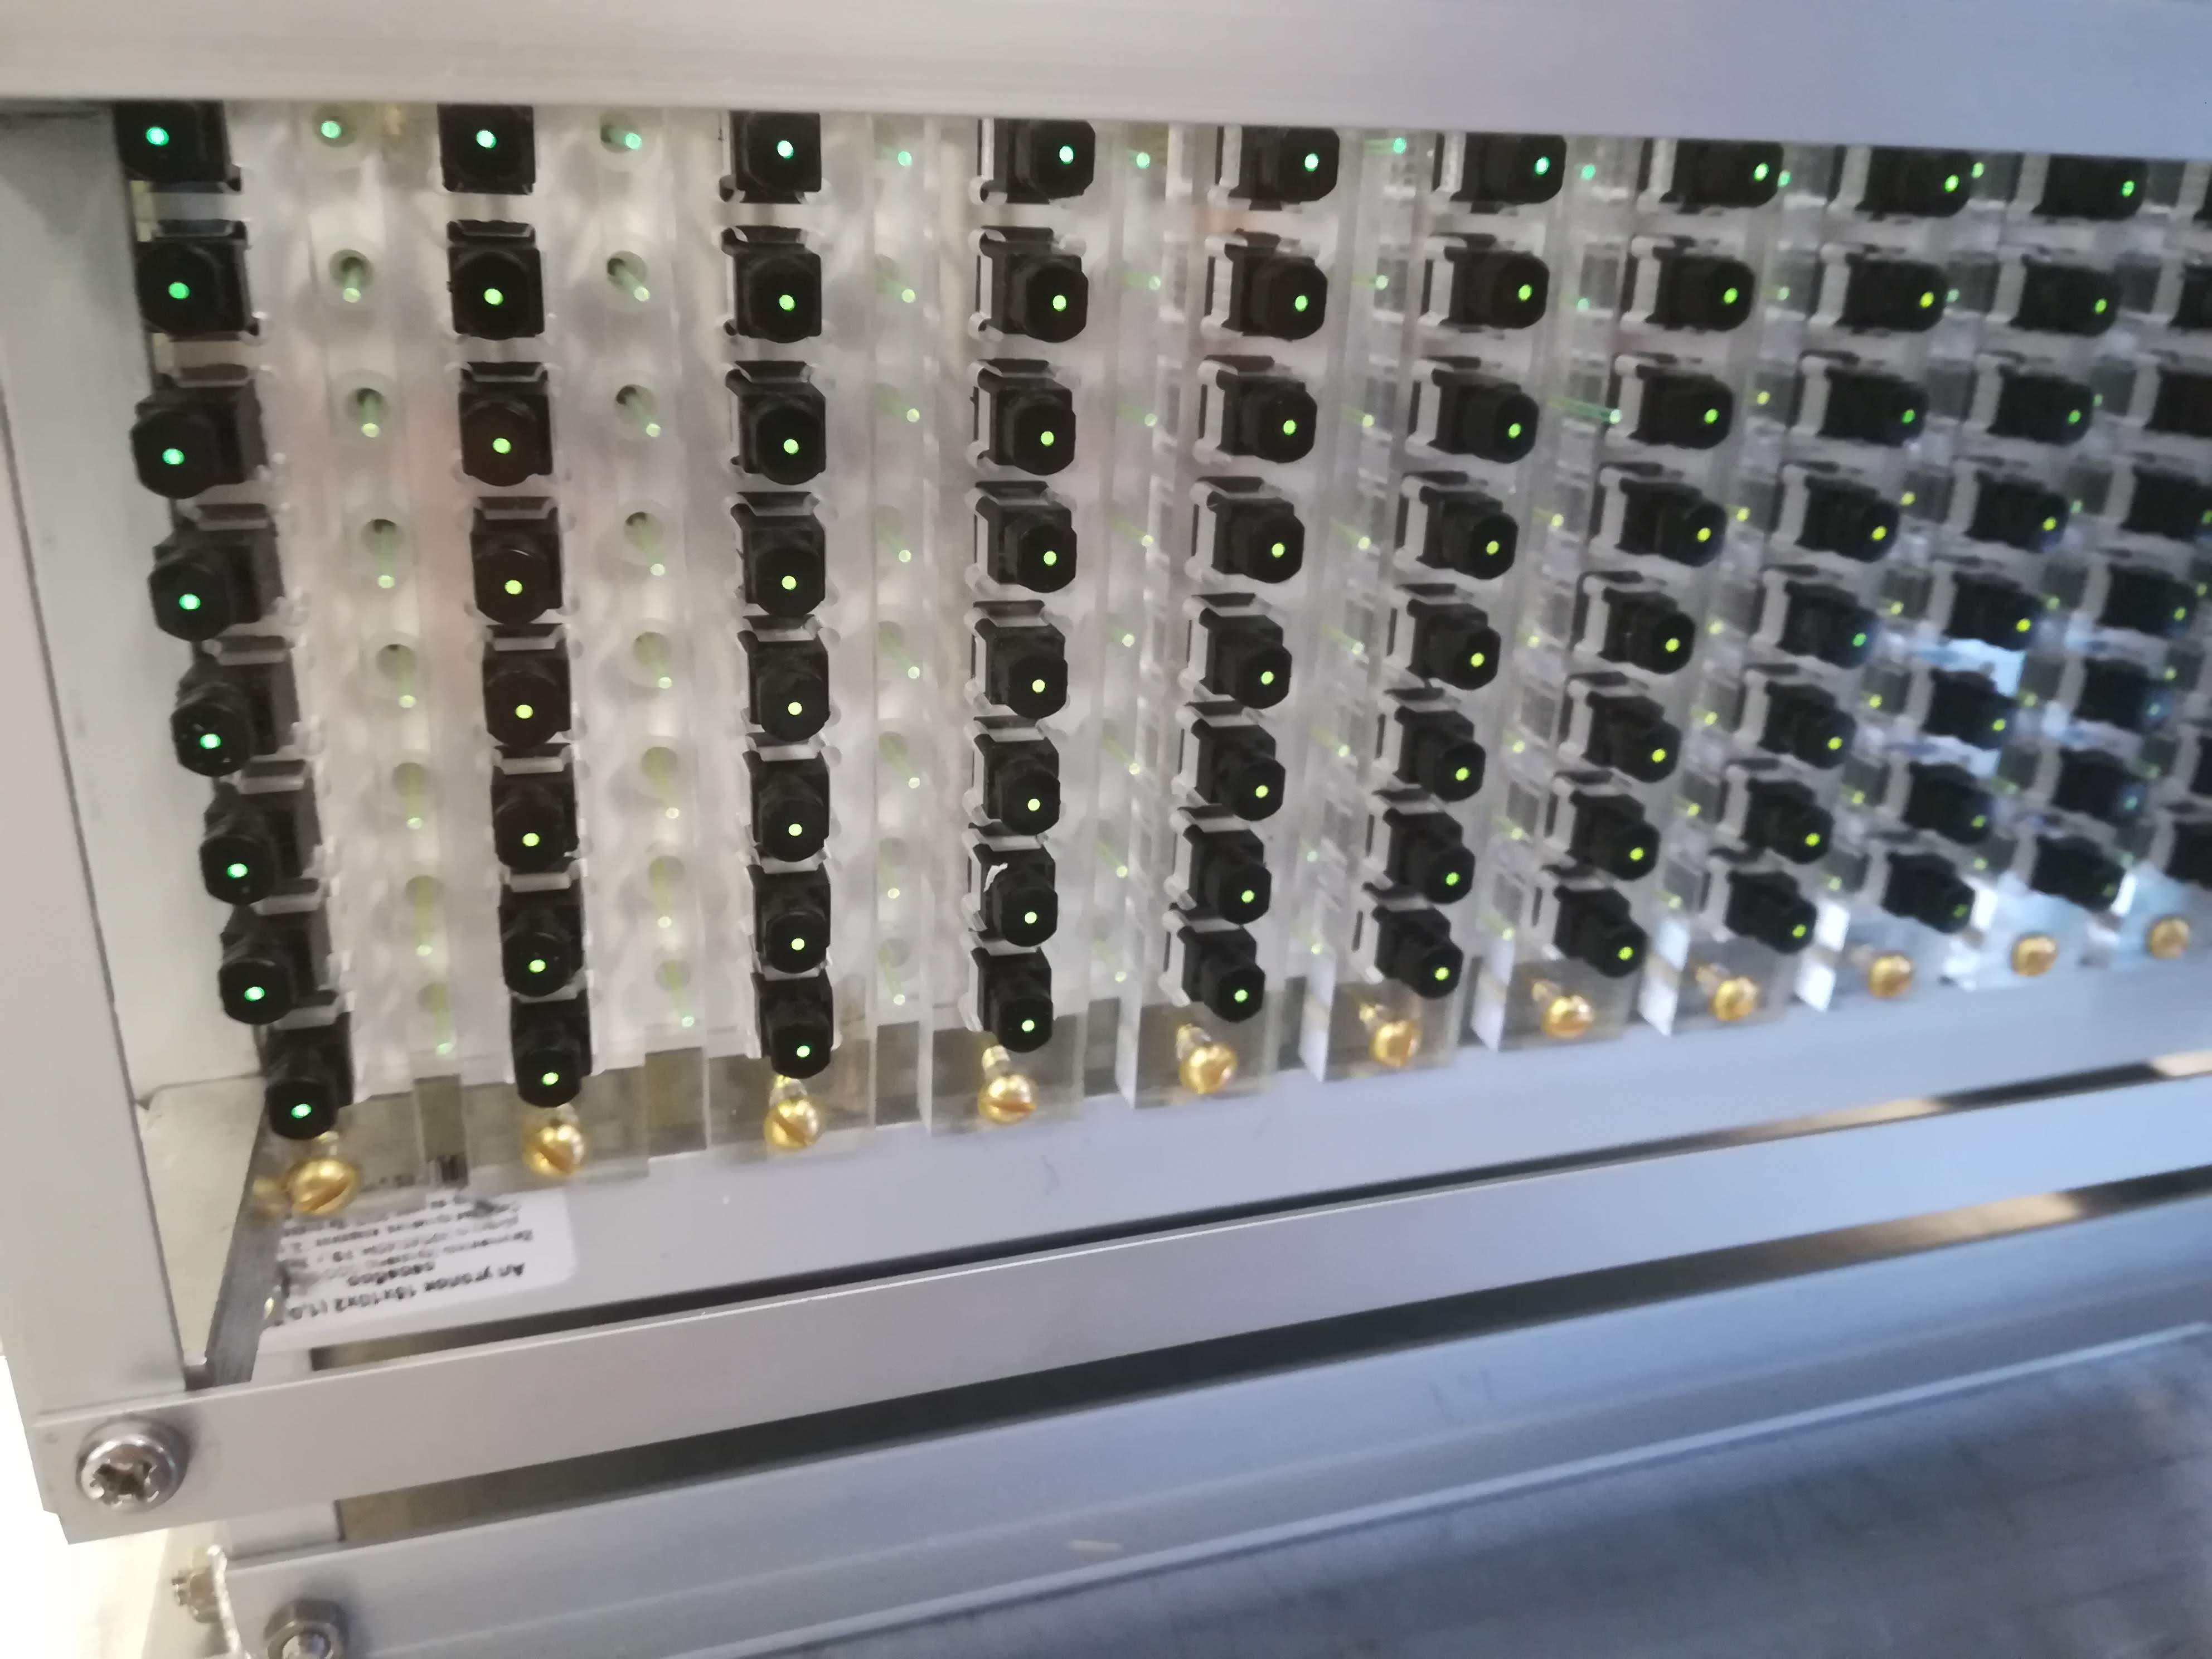
\includegraphics[width=.8\linewidth]{side}
   \caption{•}
   \label{protob}
  \end{subfigure}
  \caption{Photographs of the Super-FGD prototype after being delivered to CERN. These were taken before the electronics were fitted for the beam test. (a) shows the whole detector, along with the frame it is housed in. (b) is a close-up of one of the detector's sides, giving a clear view of the scintillator cubes and the WLS fibres. The black connectors are where the readout electronics will be attached.}
  \label{fig:proto}
 \end{figure}
one shows the construct as a whole, housed in it's frame (Fig.\ \ref{protoa}); and the other displays a close-up of the side of the detector (Fig.\ \ref{protob}).

%\subsection{Readout Electronics}

\subsection{The Beam Test Configuration} //TENSE??
The beam test is taking place in the East Area of the Proton Synchotron at CERN. Test-beam T9 is being used to fire $p, \ e^+, \ e^-, \ \pi^+, \ \pi^-, \ \mu^+$ and $\mu^-$ particles at the Super-FGD prototype with momenta ranging between 0.5--3~GeV (this is the expected momentum range for particles to be produced in the ND280 detector)~\cite{Durieu2001}. The prototype will be placed inside the MNP17 magnet, which is present for Particle Identification (PID). The readout electronics need to be placed outside the magnet field, hence long cables are needed to connect the detector to the electronics. Fig.\ \ref{fig:plat}
\begin{figure}
 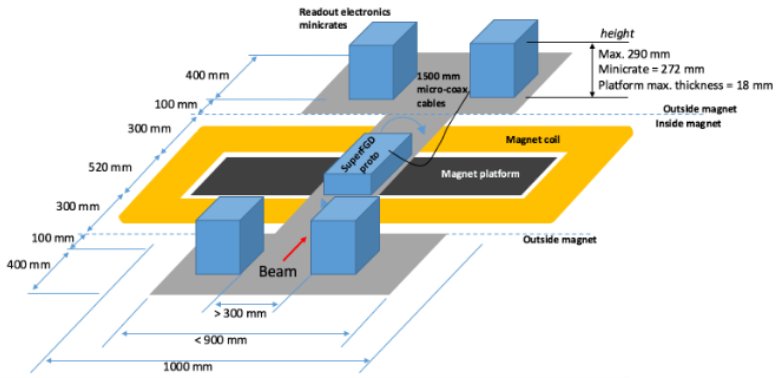
\includegraphics[scale=0.8]{platform}
 \caption{platform}
 \label{fig:plat}
\end{figure}
shows how the detector is oriented with the magnet, as well as the readout electronics, which are kept in metal boxes called ``minicrates''.

\begin{figure}
 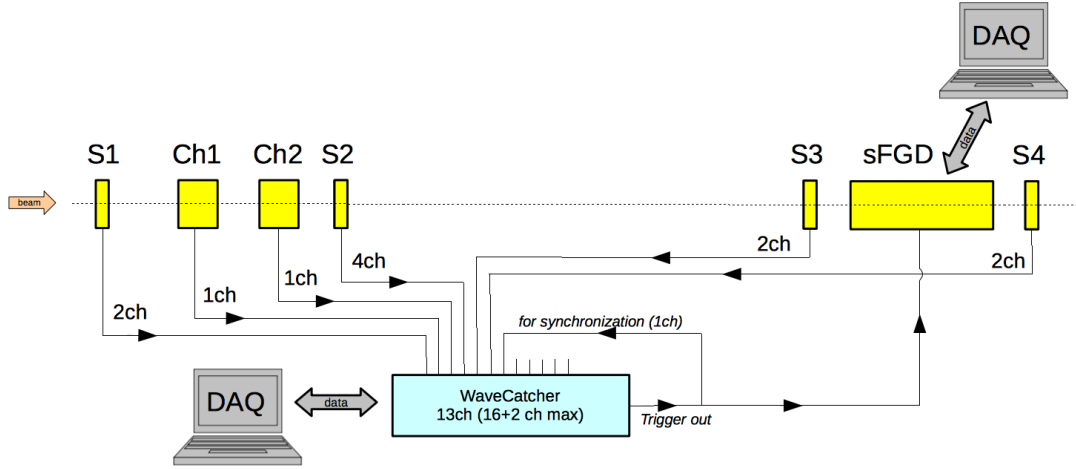
\includegraphics[scale=0.55]{daq}
 \caption{A schematic of the layout and DAQ for the beam test. The yellow boxes labelled S are beam scintillator counters and the ones labelled Ch are Cherenkov detectors. These are used in the trigger system for the Super-FGD prototype, labelled sFGD in the diagram. PID can be performed with the detectors in the triggering system by using time-of-flight and Cherenkov signals. There are two independent DAQ systems, one based on WaveCatcher, and the other BabyMIND, which is self-triggering. Also shown are the number of channels (ch) from each trigger component.}
 \label{fig:daq}
\end{figure}

\subsection{Assembling the Prototype}

\subsection{Initial Beam Test Results}

\section{Software Changes}
There have been few changes to ND280's software structure since it was conceived 14 years ago, despite many new and upgraded software tools being introduced by developers. The proposal of an upgrade to ND280's hardware has sparked discussions of updates to the software, none of which will include a major overhaul of the framework, but will help streamline the code for the modern day developer. In this section, we will outline the changes that have been proposed following discussions from the ND280 software group, some of which are still subject to certain conditions and may change later on.

\subsection{Version Control}
CVS has been the version control system (VCS) of ND280 since it was first made. Back then, there were few alternatives and CVS seemed most suited to the task. More recently, however, advances have been made in the world of VCSs, with the introduction and popularisation of distributed systems. CVS is a centralised VCS. The difference between these two is that centralised VCSs require a master repository to which developers commit changes, but distributed VCSs allow developers to ``clone'' the software and all its metadata to a repository on their own hard drive. There are several advantages of distributed VCSs, including the ability to commit several changes at once, not requiring all developers of the project to see all the changes you make and not requiring an internet connection for actions other than pulling and pushing data to other repositories. //REWORD.

Given these advantages and many others, the ND280 software will be moved to a Git-based repository. It is most likely, though, that a frozen version of the latest software version at the time of migration will be kept on CMT, as means of a back-up. It's also possible that people can still commit changes to the CVS version after the migration, which will then be ported to the Git version, though this is still undecided.

There is also the question of which Git service to use. The choice is between GitHub, a popular VCS run on a //**commercial** server, which would require a paid subscription to keep the code stored there to be kept private. Alternatively, there is GitLab, a service specifically made with scientific experiments in mind, which requires a private server to be hosted. With this VCS the software will not be viewable by anyone, and specific levels of access can be given to individuals. There is also the benefit of built in continuous integration, a feature that makes the process of editing and committing code that much faster.

There has been no official decision as to which Git service to use, although it seems that people are swaying towards the GitLab option, for its extra features and--as was CVS back in the day--structure tailor-made for scientists. This would require a private server, but the University of Warsaw, Poland, has offered to do this.

\subsection{Package Names}

COMET, another J-PARC experiment, which is searching for neutrino-less muon to electron decay, based it's software structure on that of ND280's~\cite{Wu2017}. In the process of editing the software for their specific use, they updated the package names to make them more consistent and clear. The imminent upgrade could be a good opportunity for ND280's software to follow suit, as there are some arguably confusing names and labelling rules.

A good example of COMET's updated package names is the renaming of the package elecSim to SimDetectorResponse. A developer new to the project would find it hard to discern the role of elecSim in the software (which is to simulate the electronics response of the detector), whereas SimDetectorResponse could not be much clearer. The example also highlights COMET's convention to add a prefix to each package name---such as ``Sim'' or in other cases ``Recon'', ``Calib'' and so on---that highlights where the package will be used in the data flow, i.e. in the simulation, the reconstruction, the calibration or something else. ND280 does this to an extent, but not as consistently, and a suffix is usually used rather than a prefix. 

Some other changes made by COMET were the use of capital letters. In ND280, most package names begin with lower-case lettering, but COMET have made each package begin with an upper-case letter (except packages with the ``oa'' prefix). This is a very basic change but one that arguably makes the names neater and easier to pick out in lists. A change was also made to the lettering of acronyms. For example, the package name ``fgdCalib'' in ND280 was changed to ``CalibFGD''. Again, this is a minor change but it makes the name much clearer and avoids confusion between acronyms and words.

From discussions by the ND280 software group, it seems likely that, when the software is migrated to a new VCS, the package names will be updated in a similar manner to the changes made by COMET, although the decision is not yet concrete.

\subsection{CMake and CMT}
The final applications of a software package need to be built after the software is edited or downloaded for the first time. From a developer's standpoint the performance of the build-tool is critical as they will have to build the software many times. A consumer of the software should only need to build the software applications once, so they are more concerned with the ease-of-use of the build tool. The creation and hierarchy properties of ND280's packages have so far been managed by CMT. Many other high energy physics experiments have used CMT with their software, but recently they have been switching to CMake~\cite{CMake}. One notable example is LHCb, who, until recently, maintained and used CMT before moving to CMake~\cite{Clemencic2012}.

CMake has an advantage over CMT through it's optimised code. This is especially useful on projects with a large number of packages, such as ND280, where CMT can perform significantly slower than CMake. One caveat, however, is the absence of some features that were present in CMT. The inheritance of link and compile flags, for example, is included in CMT. This is the process where, if one library (library1) is linked against another (library2), the paths to header files for library2 are included in the compile commands for library1, and all the libraries that were linked to library2 will be included in the link command to library1. In CMake, only the link command feature is included, and not the inherited paths for compile commands. This problem is surmountable because of the CMake language, which allows the construction of custom functions, including the implementation of compile flags. 

Overall, the advantages in performance most likely outweigh the work that would be required to include the missing features in CMake. Yet, there is currently still some debate as to whether ND280 should switch to CMake. It has clear advantages over CMT, but, on top of the extra effort of the implementation of features already included in CMT, many of the developers are unfamiliar with CMake, prompting the question of whether the move is worth the effort of learning the language of CMake. Currently, a few developers are attempting to build the ND280 software with CMake, and the results of their efforts will influence the decision of whether to stick with CMT or migrate to CMake.

\subsection{Mix-in Classes}
The software of ND280 currently uses ROOT5, but the latest version is ROOT6. It has been decided to update the software to integrate ROOT6, but in doing so a few things must be changed. The implementation of mix-in classes is the most notable issue. Mix-in classes are used in multiple inheritance, where the properties of several classes can be inherited. However, this is not implemented in ROOT6. The problem can be solved by replacing the implementation of the mix-in classes with C macros, but one would also need to alter the user code that accesses the mix-in classes.

To gauge how big of a job this would be, I performed a survey on the software to count the number of times mix-in classes are used (they can be identified by the ``TM'' prefix and ``State'' suffix in their name). The survey also identified the software packages and files each reference to the mix-in class was made in, but here I will only quote the final count of mix-in classes: five classes inherited a mix-in class and the mix-in classes are directly used in the code 50 times. This is relatively infrequent so the transition to ROOT6 shouldn't be significantly delayed by the reimplementation of these classes.



\section{Electron Neutrino Detection}

\subsection{Cuts}

\subsection{Analysis}

\section{Future Work}

\section{Summary}

\bibliographystyle{mystyle}
\bibliography{bibliography.bib}

\end{document}
